\chapter{逆向工程}
\section{静态分析}
\subsection{1-helloword}
打开直接F5查看伪代码得到flag:
\begin{lstlisting}
n1book{Welcome_to_reversing_world!}
\end{lstlisting}

\subsection{2-simpleCrackme}
直接查看伪代码:
\begin{lstlisting}[language=C]
int __cdecl main(int argc, const char **argv, const char **envp)
{
  size_t v3; // rbx
  int result; // eax
  char v5; // [rsp+Bh] [rbp-A5h]
  int i; // [rsp+Ch] [rbp-A4h]
  char v7[32]; // [rsp+10h] [rbp-A0h] BYREF
  char s[96]; // [rsp+30h] [rbp-80h] BYREF
  int v9; // [rsp+90h] [rbp-20h]
  unsigned __int64 v10; // [rsp+98h] [rbp-18h]

  v10 = __readfsqword(0x28u);
  strcpy(v7, "zpdt{Pxn_zxndl_tnf_ddzbff!}");
  memset(s, 0, sizeof(s));
  v9 = 0;
  printf("Input your answer: ");
  __isoc99_scanf("%s", s);
  v3 = strlen(s);
  if ( v3 == strlen(v7) )
  {
    for ( i = 0; i <= strlen(s); ++i )
    {
      if ( s[i] <= 96 || s[i] > 122 )
      {
        if ( s[i] <= 64 || s[i] > 90 )
          v5 = s[i];
        else
          v5 = (102 * (s[i] - 65) + 3) % 26 + 65;
      }
      else
      {
        v5 = (102 * (s[i] - 97) + 3) % 26 + 97;
      }
      if ( v5 != v7[i] )
      {
        puts("Wrong answer!");
        return 1;
      }
    }
    puts("Congratulations!");
    result = 0;
  }
  else
  {
    puts("Wrong input length!");
    result = 1;
  }
  return result;
}
\end{lstlisting}

首先有字符串:'zpdt\{Pxn\_zxndl\_tnf\_ddzbff!\}',需要构造一个输入字符串来满足要求,输入字符串首先会检查总长度是否和目标串一致,而后会逐字符经过一个运算后检查结果是否和给定字符串同样位置的字符一致。运算流程为:
\begin{enumerate}
    \item 若不是字母,则不变,直接比较。
    \item 若是大写字母,则$res = (102 \times (v - 65) + 3) \%26 + 65$。
    \item 若是小写字母,则$res = (102 \times (v - 97) + 3) \%26 + 97$。
\end{enumerate}
直接写个脚本暴力求解:
\begin{lstlisting}[language=python]
def crack(a):
    res = 0
    if a <= 96 or a > 122:
        if a <= 64 or a > 90:
            res = a
        else:
            res = (102 * (a - 65) + 3) % 26 + 65
    else:
        res = (102 * (a - 97) + 3) % 26 + 97;
    return res

if __name__ == '__main__':
    target = 'zpdt{Pxn_zxndl_tnf_ddzbff!}'
    ans = ''
    for i in range(len(target)):
        for j in range(0,250):
            if chr(crack(j)) == target[i]:
                ans += chr(j)
                break
    print(ans)
\end{lstlisting}
获得结果:chaf\{Hdi\_cdiaj\_fim\_aacbmm!\},输入目标程序后得到输出:'Congratulations!'。解题完成。

\section{动态分析}

\subsection{2-simpleCrackme\_O3}
是上一题的经过编译器优化的版本,仅目标字符串解析出来有问题,需要手动设置为char[28]数组。

\subsection{3-upx}
脱壳题。原程序用ida打开只有一个start函数,生成的伪代码也只有这个函数的内容。

用x64DBG一打开是ntdll里面的代码,按F9运行,到程序入口点后会自动停下,发现入口点就是一个pushad,那么在pushad后下一个硬件读取断点(右键右边寄存器区域,设置硬件断点于ESP)。

继续运行,运行到popad指令后断点被触发~\ref{fig:5_pic1},此时删除断点。发现popad之后在循环清空栈上方区域,之后跳转到了一个比较远的地址。
\begin{figure}[H]
    \centering
    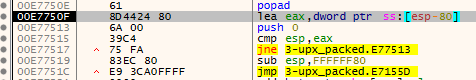
\includegraphics[width=0.8\textwidth]{5-reverse_engineering/pic/1.jpg}
    \caption{popad}
    \label{fig:5_pic1}
\end{figure}

跟进该地址,发现看起来像一个正常函数,然后按步骤导出脱壳程序即可。这个脱壳程序已经可以用ida打开并解析出来了,但是还不能运行。需要禁用ASLR,用CFF Explorer修改修改Nt Header的"Charatristics",勾选"Relocation info stripped from file",最后发现这个方法无效,直接修改平台给的dump程序也不能运行,不知道是哪里有问题。